\documentclass[aspectratio=169]{beamer}
\usepackage{amsmath}
\usepackage{amssymb}
\usepackage{tikz}
\usepackage{fancyvrb}
\usepackage{xcolor}
\title{Symbolic Execution with Angr\\RPISEC}
\date{December 6, 2019}
\author{Avi Weinstock (\Verb|aweinstock|), Luke Biery (\Verb|tiecoon|)}

\definecolor{rpisecbgcolor}{RGB}{21, 24, 32} % 151820
\definecolor{cybercyan}{RGB}{42, 171, 219} % 2aabdb
\definecolor{cybergreen}{RGB}{106, 220, 169} % 6adca9
\definecolor{cyberpink}{RGB}{248, 106, 140} % f86a8c

\setbeamercolor{normal text}{fg=white}
\setbeamercolor{frametitle}{fg=cybercyan}
\setbeamercolor{title}{fg=cybercyan}
\setbeamercolor{structure}{fg=cybercyan}

%>>> [0x15,0x18,0x20]
%[21, 24, 32]
% convert rpisec_background.png -alpha set -fill '#15182080' -draw 'rectangle 0 0 1090 1216' rpisec_background2.png
% convert probable_prime.png -alpha set -fill '#151820c0' -draw 'rectangle 0 0 414 836' probable_prime2.png
\usebackgroundtemplate{
\colorbox{rpisecbgcolor}{\raisebox{1pt}[\paperheight][\depth]{\hspace{0.6\paperwidth}
%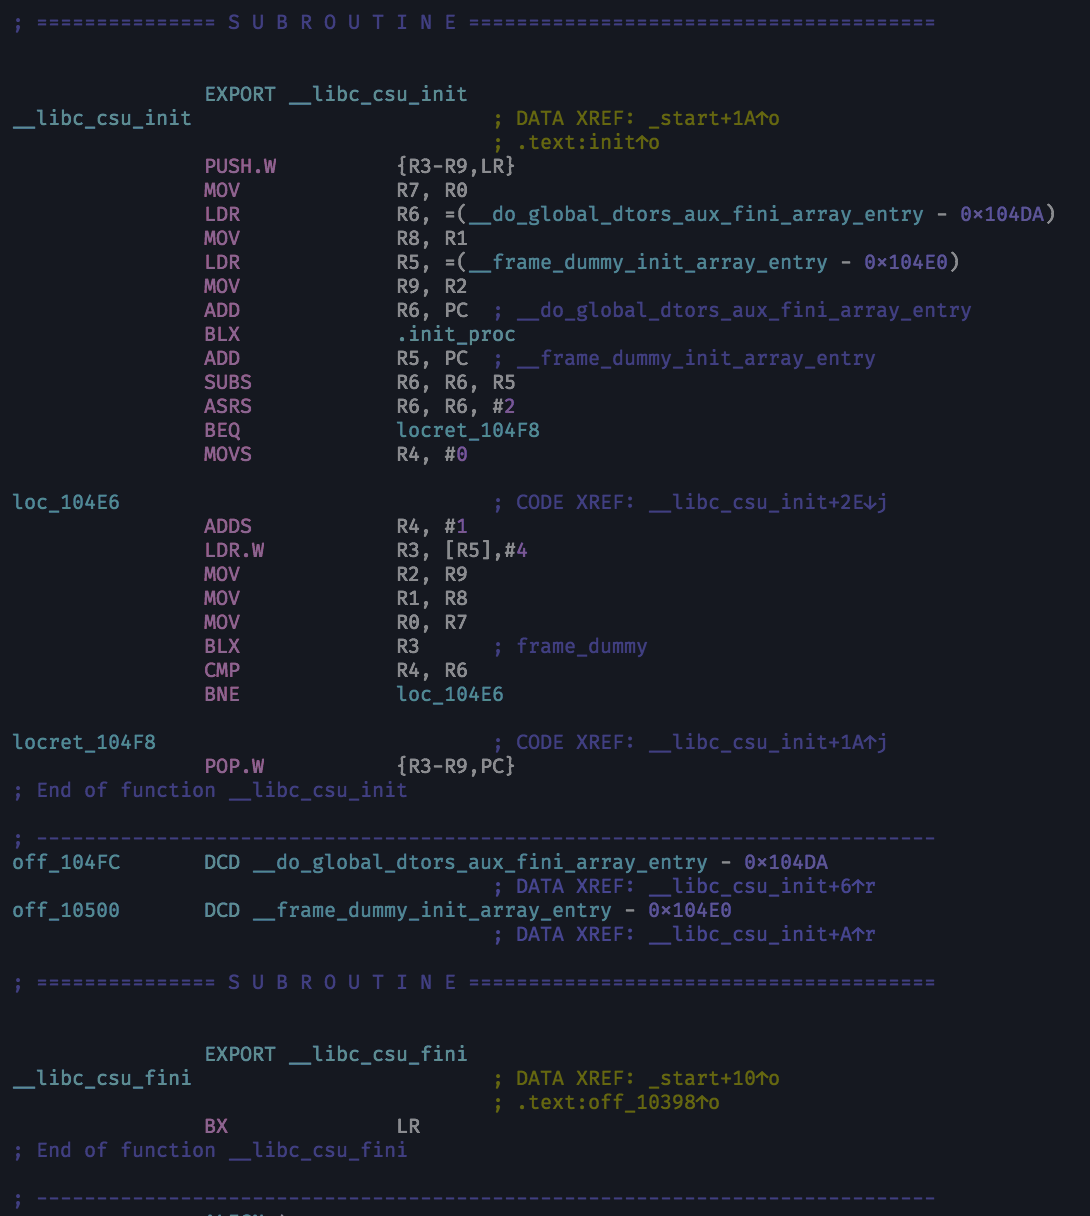
\includegraphics[width=0.4\paperwidth, height=\paperheight]{rpisec_background2.png}
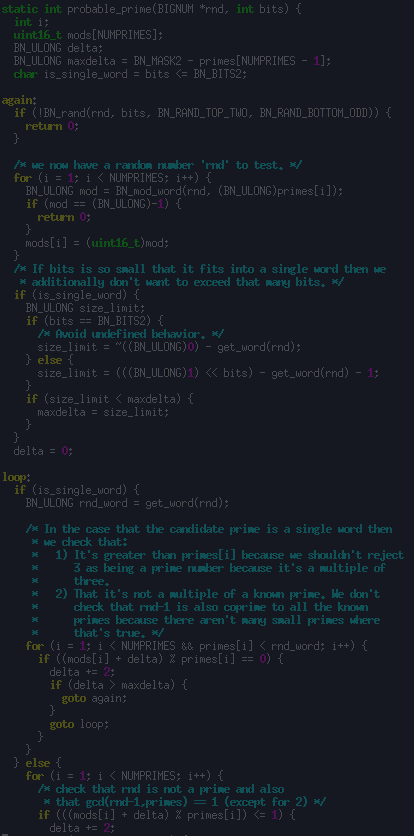
\includegraphics[width=0.4\paperwidth, height=\paperheight]{../rsa_2019_10_29/probable_prime2.png}
}}
}

\newcommand{\SlideWithCenteredText}[1]{
  \begin{frame}
  \vfill
  \centering
  \begin{beamercolorbox}[sep=8pt,center,shadow=true,rounded=true]{title}
    \usebeamerfont{title}#1\par%
  \end{beamercolorbox}
  \vfill
  \end{frame}
}

\newcommand{\questionsslide}[1]{\SlideWithCenteredText{Any questions#1?}}

% https://tex.stackexchange.com/questions/178800/creating-sections-each-with-title-pages-in-beamers-slides
\AtBeginSection[]{
\SlideWithCenteredText{\insertsectionhead}
}



\begin{document}
\maketitle

\begin{frame}[fragile]
\frametitle{Overview}
\begin{itemize}
\item What is Symbolic Execution? What techniques does it compete with?
\item How symbolic execution works (theory)
\item How symbolic execution works (Angr commands)
\item Solving MBE lab1A with Angr
\end{itemize}
\end{frame}

\section{Background - What it is and what is the problem space?}
\begin{frame}[fragile]
\frametitle{What is Symbolic Execution?}
\begin{itemize}
\item Executes a program with symbolic data (usually input)
\item Essentially runs a program on "all possible inputs" at once
\item Instead of having concrete data in each variable/address, \\variables/addresses store trees of what to do with the input
\end{itemize}
\end{frame}

\begin{frame}[fragile]
\frametitle{What problems does Symbolic Execution solve?}
\begin{itemize}
\item What input to provide to reach/avoid a specific line of code?
\item How is a value deep in the program affected by some specific input?
\item Do any inputs lead to any crash?
\item On a crashing input, what registers are controlled by the input?
\end{itemize}
\end{frame}

\begin{frame}[fragile]
\frametitle{Symbolic Execution vs Fuzzing}
\begin{tabular}{c|c}
Symbolic Execution & Fuzzing\\\hline
\textcolor{green}{+ Explores all inputs} & \textcolor{red}{- Only explores random inputs}\\
\textcolor{red}{- Uses more memory/time} & \textcolor{green}{+ Uses around as much memory/time as target program}
\end{tabular}
TODO: more comparisons/columns? emphasize that "all inputs" means that symexec can find constant-time comparisons against a giant constant, unlike coverage-guided?
\end{frame}

\section{How symbolic execution works in general}

\begin{frame}[fragile]
\frametitle{Setting up a state for symbolic execution}
\begin{itemize}
\item \begin{Verbatim}[fontsize=\scriptsize, frame=single]
import z3
registers = ['eax', 'ebx', 'ecx', 'edx', 'ebp', 'esp'] # and so on
symstate = {reg: z3.BitVec(reg, 32) for reg in registers}
symstate['memory'] = z3.Array('memory', z3.BitVecSort(32), z3.BitVecSort(8))
\end{Verbatim}
\item Note that the z3 variable \verb|eax| in the model will be the starting value of \verb|eax|
\item \verb|symstate['eax']| will be mutated throughout the computation, and will contain an expression corresponding to the ending value of \verb|eax|
\end{itemize}
\end{frame}

\begin{frame}[fragile]
\frametitle{Symbolically executing branch-free code}
\begin{itemize}
\item Translate arithmetic, indexing, etc into SMT constraints
\end{itemize}
\begin{minipage}{0.3\textwidth}
\begin{Verbatim}[fontsize=\scriptsize, frame=single]
mov eax, ebx
\end{Verbatim}
\end{minipage}
\begin{minipage}{0.68\textwidth}
\begin{Verbatim}[fontsize=\scriptsize, frame=single]
symstate['eax'] = symstate['ebx']
\end{Verbatim}
\end{minipage}

\begin{minipage}{0.3\textwidth}
\begin{Verbatim}[fontsize=\scriptsize, frame=single]
add ecx, edx
\end{Verbatim}
\end{minipage}
\begin{minipage}{0.68\textwidth}
\begin{Verbatim}[fontsize=\scriptsize, frame=single]
symstate['ecx'] += symstate['edx']
\end{Verbatim}
\end{minipage}

\begin{minipage}{0.3\textwidth}
\begin{Verbatim}[fontsize=\scriptsize, frame=single]
mov byte [esp+0x10], al
\end{Verbatim}
\end{minipage}
\begin{minipage}{0.68\textwidth}
\begin{Verbatim}[fontsize=\scriptsize, frame=single]
esp_10 = symstate['esp']+0x10
al = z3.Extract(7, 0, symstate['eax'])
symstate['memory'] = z3.Store(symstate['memory'], esp_10, al)
\end{Verbatim}
\end{minipage}

\begin{minipage}{0.3\textwidth}
\begin{Verbatim}[fontsize=\scriptsize, frame=single]
movsx eax, byte [eax]
\end{Verbatim}
\end{minipage}
\begin{minipage}{0.68\textwidth}
\begin{Verbatim}[fontsize=\scriptsize, frame=single]
star_eax = z3.Select(symstate['memory'], eax)
symstate['eax'] = z3.SignExt(24, star_eax)
\end{Verbatim}
\end{minipage}
\end{frame}

\begin{frame}[fragile]
\frametitle{TODO: Avi}
\begin{itemize}
\item symbolic branches
\item symbolic loops
\item symbolizing tainted memory (e.g. \verb|sym_memory[(EBP+username+i)]| vs \verb|sym_username[i]|)
\item state explosion when looping on symbolic data
\end{itemize}
\end{frame}

\section{How to use Angr for symbolic execution}
\begin{frame}[fragile]
\frametitle{TODO: Luke}
\begin{itemize}
\item loading binariess
\item marking input as symbolic
\item initiating the search/pruning the search space
\item simprocedures for shortcutting syscalls?
\end{itemize}
\end{frame}

\section{Example: MBE lab1A with Angr}
\begin{frame}[fragile]
\frametitle{Resources}
\begin{itemize}
\item \verb|https://github.com/angr/|
\item \verb|https://github.com/Z3Prover/z3/|
\item \verb|https://github.com/RPISEC/MBE|
\end{itemize}
\end{frame}
\end{document}
